% !TEX root = ../Article.tex
\chapter{Background}
In this chapter we will provide background information necessary to understand how smart cards function and can increase security on mobile devices. The topics covered in this section are smart cards, mobile device operating systems, cryptography and threats in context of mobile devices.

\section{Terminology}
\paragraph{APDU}
Application Protocol Data Unit describes the format of how a smart card and other applications should communicate. Refer to section \ref{sec:communicationstandard}.

\paragraph{Extended APDU}
Extended Application Protocol Data Unit is an extension of an Application Protocol Data Unit where the payload data supports lengths up to 65535 bytes.

\paragraph{SELECT APDU}
SELECT APDU is a type of APDU that has the sole purpose of activating the correct application on the smart card.

\paragraph{Application Identifier (AID)}

\section{Smart Card}
\label{sec:smartcard}
A smart card refers to a pocket sized card with an integrated circuit, usually in the form of a plastic card with an integrated micro processor. In essence a smart card is a miniature computer with limited computing power.

\subsection{Smart card architecture}
The micro processor is able to perform tasks that involve processing input, give ouput and storing small amounts of data. Smart cards vary in sizes defined by the standards ISO/IEC 7810 \cite{iso7810} and ISO/IEC 7816 \cite{iso7816}. The processing power of smart cards are between 25-32 MHz and sport anywhere from 8Kbit to 128Kbit memory (EEPROM) \cite{cardProcessing}.

The micro processor can be powered and communicate in two ways. Contact smart cards have integrated contact pads. When the smart card is inserted into a card reader the contact pads of the card reader provides power to the micro processor via the contact pads of the smart card. The contact pads also works as a medium for transferring data. Contactless smart cards uses radio-frequency induction to power the micro processor and to transmit data between an antenna and the card. Most modern cards support both of these technologies. Figure \ref{fig:nfccard} is a blank hybrid card.

An everyday example of a smart card is the modern credit and debit card. Most of these cards are contact cards that require the user to insert the card into a card reader, but newer cards are of the hybrid type, that have the ability to communicate over radio frequencies. Credit and debit cards utilizes the input/output capabilities of the smart card, but they also store information on the card authenticating the users bank information.

\begin{figure}[h!]
  \caption{Hybrid Smart card.}
  \label{fig:nfccard}
  \centering
    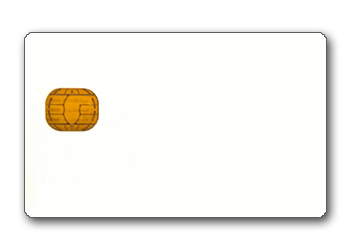
\includegraphics[width=0.75\textwidth]{images/nfccard2.png}
\end{figure}

\subsection{Communication standard for smart cards}
\label{sec:communicationstandard}
Application Protocol Data Unit (APDU) is a standard that describes how a smart card application should communicate with other applications (off-card) and is defined by ISO7816-4 \cite{iso7816-4}. There are two types of APDU messages: Command APDU and Response APDU.

Command APDU is split into header and body. Refer to table \ref{tbl:cmdAPDU} for instruction explanation and summary. The header is mandatory for all transactions and consists of 4 bytes that is split into CLA, INS, P1 and P2. The body of a command APDU is split into 3 parts; LC, Payload and LE. LC is 1 byte, payload is maximum 255 bytes and LE is 1 byte.

Newer smart cards supports Extended APDU which allows the payload to be up to a maximum of 65535 bytes. If the payload data is greater than 255 bytes LC must be 3 bytes where the first byte is 0x00 to denote that the APDU is extended and the remaining bytes denotes the length. If extended APDU is used then LE consists of 2 bytes to account for longer responses.
\begin{table}[h!]
\caption{Command APDU layout.}
\label{tbl:cmdAPDU}
\centering

    \begin{tabular}{ | l | c | l |}
        \hline
        \thead{Name}
        & \thead{Number of bytes}
        & \thead{Description} \\ \hline

        CLA  & 1 & Command type class, type of command \\ \hline
        INS & 1 & Instruction code, command to run \\ \hline
        P1 & 1 & Free parameter \\ \hline
        P2 & 1 & Free parameter \\ \hline
        LC & 0, 1 or 3 & Length of payload \\ \hline
        Payload & 0 - 65535 & Payload data \\ \hline
        LE & 0, 1 or 2 & Expected response length \\ \hline

    \end{tabular}

\end{table}


Response APDU is split into body and response trailer. The body consist of the response data and is at maximum 255 bytes or 65535 bytes depending on if extended APDU is used. All response APDUs must contain a response trailer of two bytes which denotes the processing status (error, success, wrong format, etc.) of the command APDU. Refer to table \ref{tbl:rspAPDU} for definitions and summary.
\begin{table}[h!]
\caption{Response APDU layout.}
\label{tbl:rspAPDU}
\centering

    \begin{tabular}{ | l | c | l |}
        \hline
        \thead{Name}
        & \thead{Number of bytes}
        & \thead{Description} \\ \hline

        Response & 0-65535 & Response data \\ \hline
        SW1+SW2 & 2 & Command processing status \\ \hline

    \end{tabular}

\end{table}


To better understand when to use the command APDUs and when to use response APDUs we will describe the following example: A locked door has a card reader connected to it. A person walks up to the door and holds up his contactless smart card to the reader. The card reader sends a command APDU to the card asking for the ID. The smart card processes the command APDU and sends a response APDU back to the card reader containing the ID of the person. This example is visualized by figure \ref{fig:doornfc}.

\begin{figure}[h!]
  \caption{Door lock using smart card to unlock.}
  \label{fig:doornfc}
  \centering
    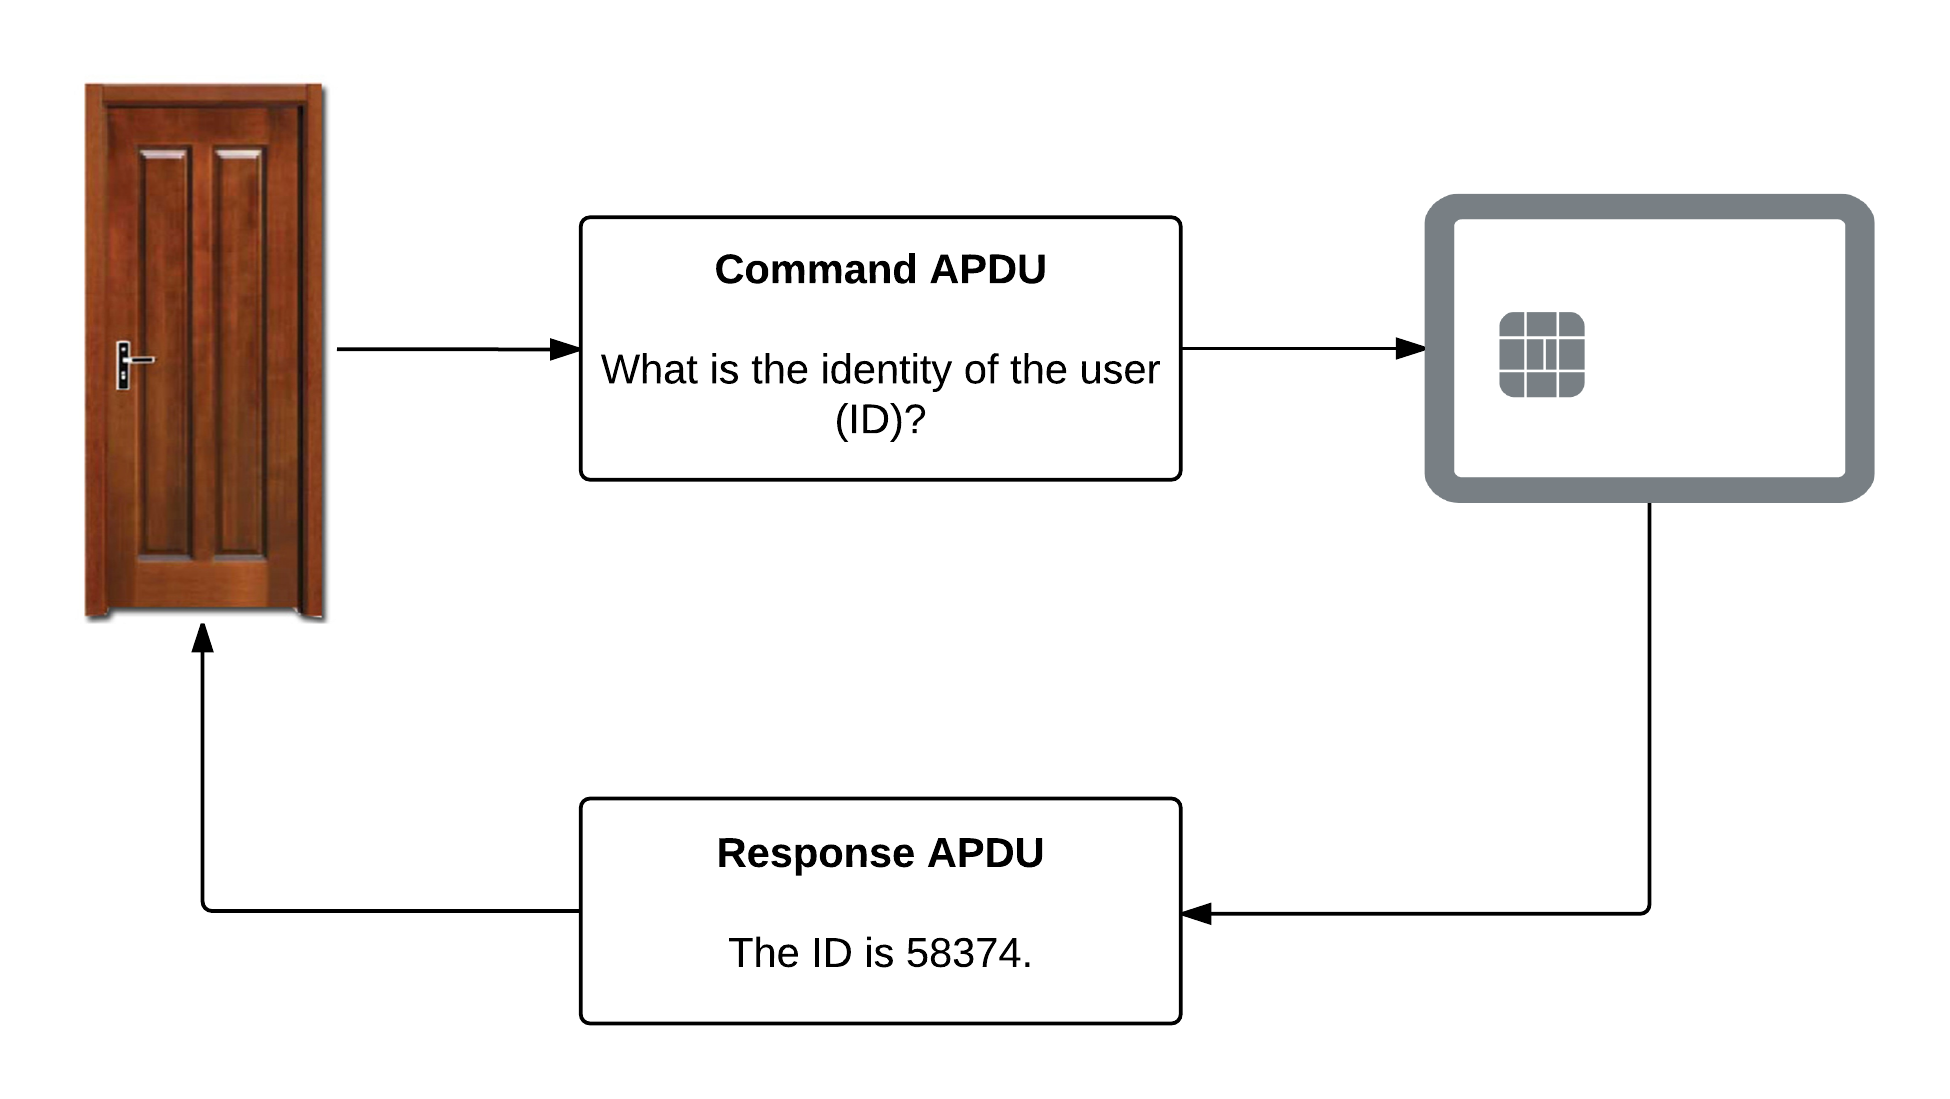
\includegraphics[width=0.95\textwidth]{images/doornfc.png}
\end{figure}

\subsection{JavaCard programming language}
\label{sec:javacard}
In section \ref{sec:smartcard} we described that smart cards are able to store data as well as process input and output. All smart cards have their own operating system that allows developers to write applications that run on the smart cards. Smart cards are not limited to one applications per card, but are able to have multiple applications installed. Traditionally it was not feasable to create programs that ran on different smart card manufacturer cards as the micro processors were manufacturer specific \cite{javacardapplet}. This created an environment where smart card issuers and their developers were locked to a specific manufacturer.

The company Schlumberger \cite{schlumberger}, later joined by Sun Microsystems \cite{sunMicroSystems}, outlined Java Card 1.0. Java Card were to alleviate the problem of manufacturer specific code and to let developers write generic applications. Newer Java Card version includes a development kit that provides a test environment and a converter tool that prepares the Java Card applet/program for installation onto a smart card. The newest Java Card version is currently 3.0.5 \cite{javacard305}.

The Java Card language behaves very similar to standard Java, but there are some substantial differences. Many Java classes and features are not present, e.g., int, double, long, java.lang.SecurityManager, threading and object cloning \cite{javacardlimits}. The structure of the applets differ from standard Java applets. All Java Card applets must implement:
\begin{itemize}
    \item \texttt{void install (byte [] barray, short bOffset, byte bLength)}
    \item \texttt{void process(APDU apdu)}.
\end{itemize}
\texttt{Install} is invoked when the applet is downloaded onto the smart card and should register and initialize the applet \cite{javacardinstall}. \texttt{Process} is the entry point for all requests to the application and where the applet specific logic is done \cite{javacardprocess}.

Garbage collection in the Java Card language differs from standard Java. In standard Java garbage collection is performed by the Java Virtual Machine (JVM) and runs independently of the application. In Java Card objects are stored in the persistent memory (EEPROM) and writing to this memory is very time-consuming. As a result it was decided that there is no automatic garbage collection in Java Card and that garbage collection must be invoked by the application itself. Deciding when to perform garbage collection is very difficult as on one side you don't want to do it often, and on the other side if you run out of memory you are out of luck.

When incorporating the features of a smart card with a mobile device it would be beneficial to not rely on an external contact card or contactless card. One of the key features of the Java Card language is that the software is able to run on technological different smart cards. As such it is possible to deploy the Java Card applet to special micro SD memory cards. This essentially enables the smart card to be integrated with the mobile device, but at the same time be an external runtime environment. Figure \ref{fig:msdcard} is a micro SD memory card produced by Gemalto.

\begin{figure}[h!]
  \caption{Micro SD card from Gemalto.}
  \label{fig:msdcard}
  \centering
    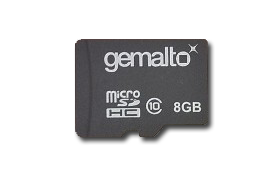
\includegraphics[width=0.75\textwidth]{images/msd.png}
\end{figure}

\subsection{Java Card versions}
\paragraph{Java Card 2.2.2}\mbox{}\\
In section \ref{sec:javacard} we discussed some of the limitations of java card
Java card 3.0.5 %TODO FIX ME PLZ



\subsection{Other smart card programming languages}
There exists several other languages for smart card programming. The two most notable are JavaCard (section \ref{sec:javacard}) and MULTOS \cite{multos}. The latter uses the programming language C as the language for writing applications.

\section{Mobile operating system}
Mobile operating system refers to the operating system running on a mobile device (smartphones, GPS devices, tablets, etc). In this thesis we will focus mainly on smartphones and tablets since their capabilities are within our scope and the fact that they often share the same operating system.

\subsection{Android}
Android is an open source licensed mobile operating system and is based on one of the LTS (long-term support) branches of the Linux kernel. Google inc. \cite{google} is the current developer of the mobile operating system and their primary focus has been smartphones and tablets. In later years Google has put resources into incorporating Android with TVs, wrist watches and cars. In 2015 Q2 82,8 \% of smartphones worldwide was shipped with a version of the Android mobile operating system \cite{androidMarketShare}.

The Android mobile operating system supports applications that are written in Java, GO and C/C++. The applications run in their own sandbox with their own allocated memory space, but applications can also access shared resources given permission to do so by the user.

\section{Cryptography}
%What is cryptography?
Cryptography is a method for protecting confidential data using complex mathematics and computer science. Most cryptographic functions/algorithms relies heavily on the fact that the mathematics are so complex that they are "uncrackable" without knowledge of the encryption/decryption key.

\subsection{Public-key cryptography}
Public-key cryptography refers to a set of methods for asymmetric cryptography. It is based around the concept that one entity (user, server, etc.) generates a key pair consisting of one public key and one private key. Data encrypted using the public key can only be decrypted by the private key and due to the complexity of the keys it is improbable that the private key can be generated from the public key. The public key, as the name suggests, is publicly available for other entities. This combination allows entities to communicate securely given that they have each others public key and their private key is stored securely. Figure \ref{fig:encrypt_basic} shows how a sender can send a message that only the receiver can read. Although it is important to note that this operation is more resource intensive and time consuming compared to symmetric key encryption/decryption.

\begin{figure}[h!]
  \captionsetup{justification=centering,margin=1.5cm}
  \caption{Asymmetric key encryption/decryption using public-private key pair.}
  \label{fig:encrypt_basic}
  \centering
    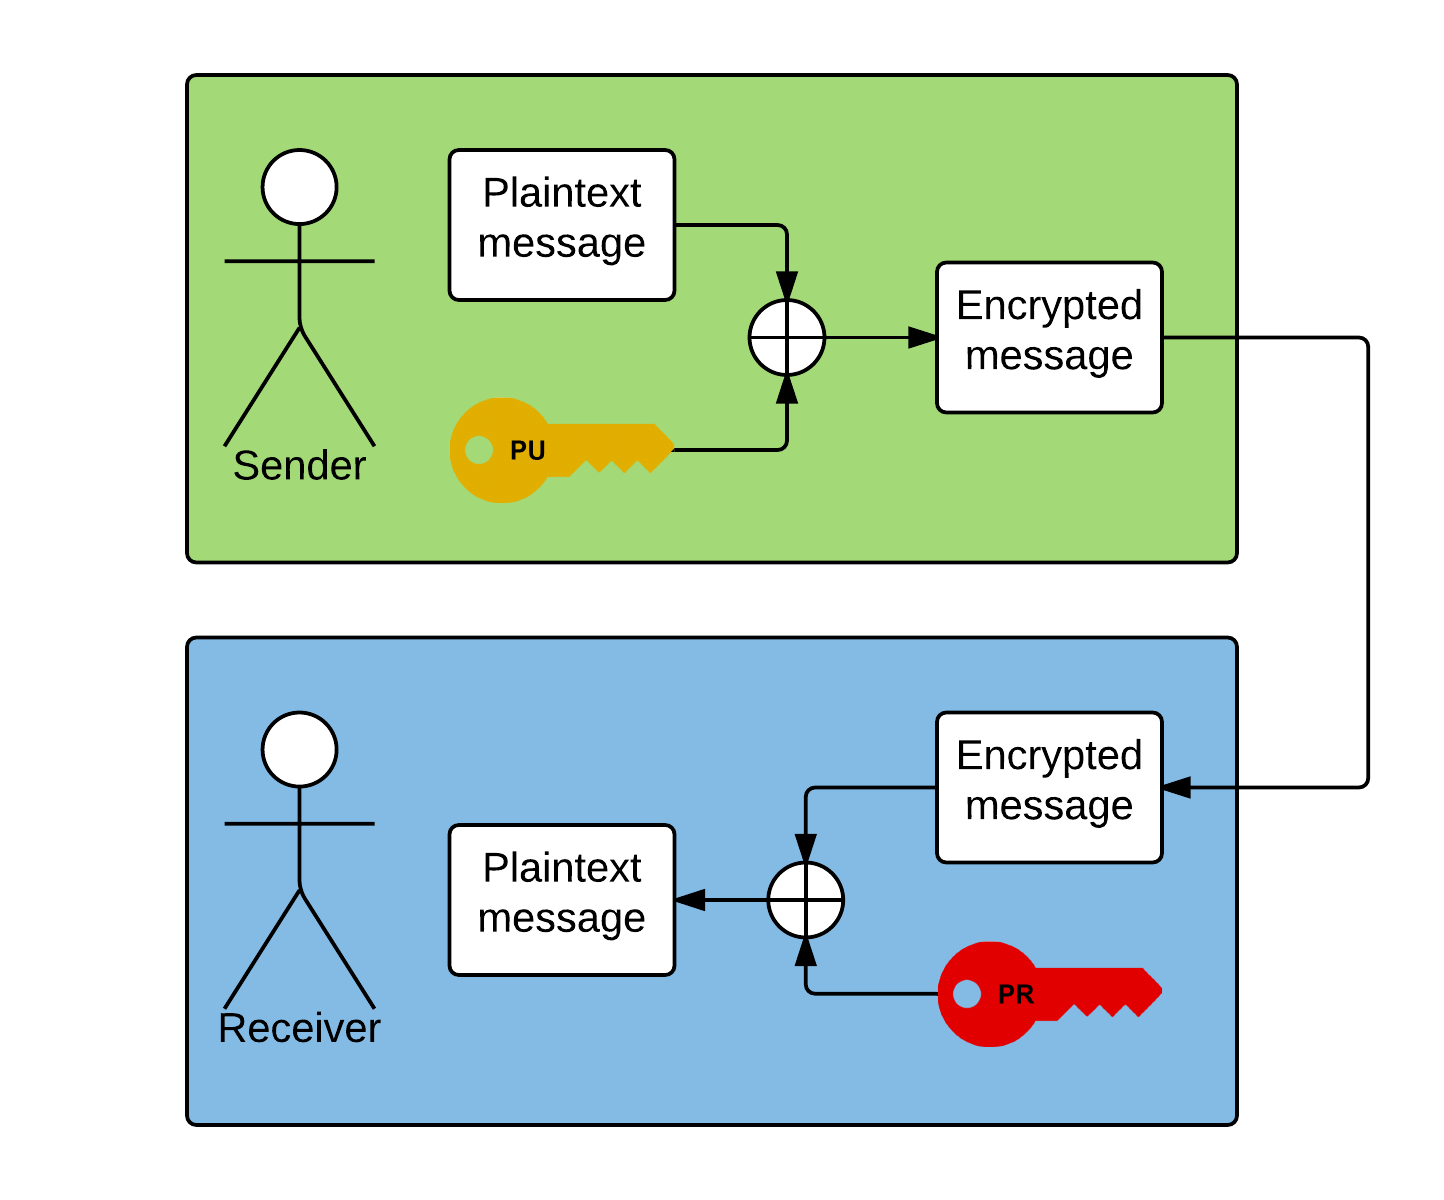
\includegraphics[width=1\textwidth]{images/encrypt_basic.png}
\end{figure}

Message authentication can also be done by public-key cryptography. First the message is hashed using a secure hash function, for instance SHA-2 \cite{shaRFC}, which creates a digest. The digest is then encrypted with the private key and the "digital signature" is then sent with the original message. The receiver can then verify the integrity of the message by computing the hash of the message using the same secure hash function and decrypt the "digital signature" using the senders public key. If they are a match the message the receiver can with certainty conclude that the message has not been tampered with and originates from the sender.

\begin{figure}[h!]
  \captionsetup{justification=centering,margin=1.5cm}
  \caption{Digital signing using public-private key pair.}
  \label{fig:signing_basic}
  \centering
    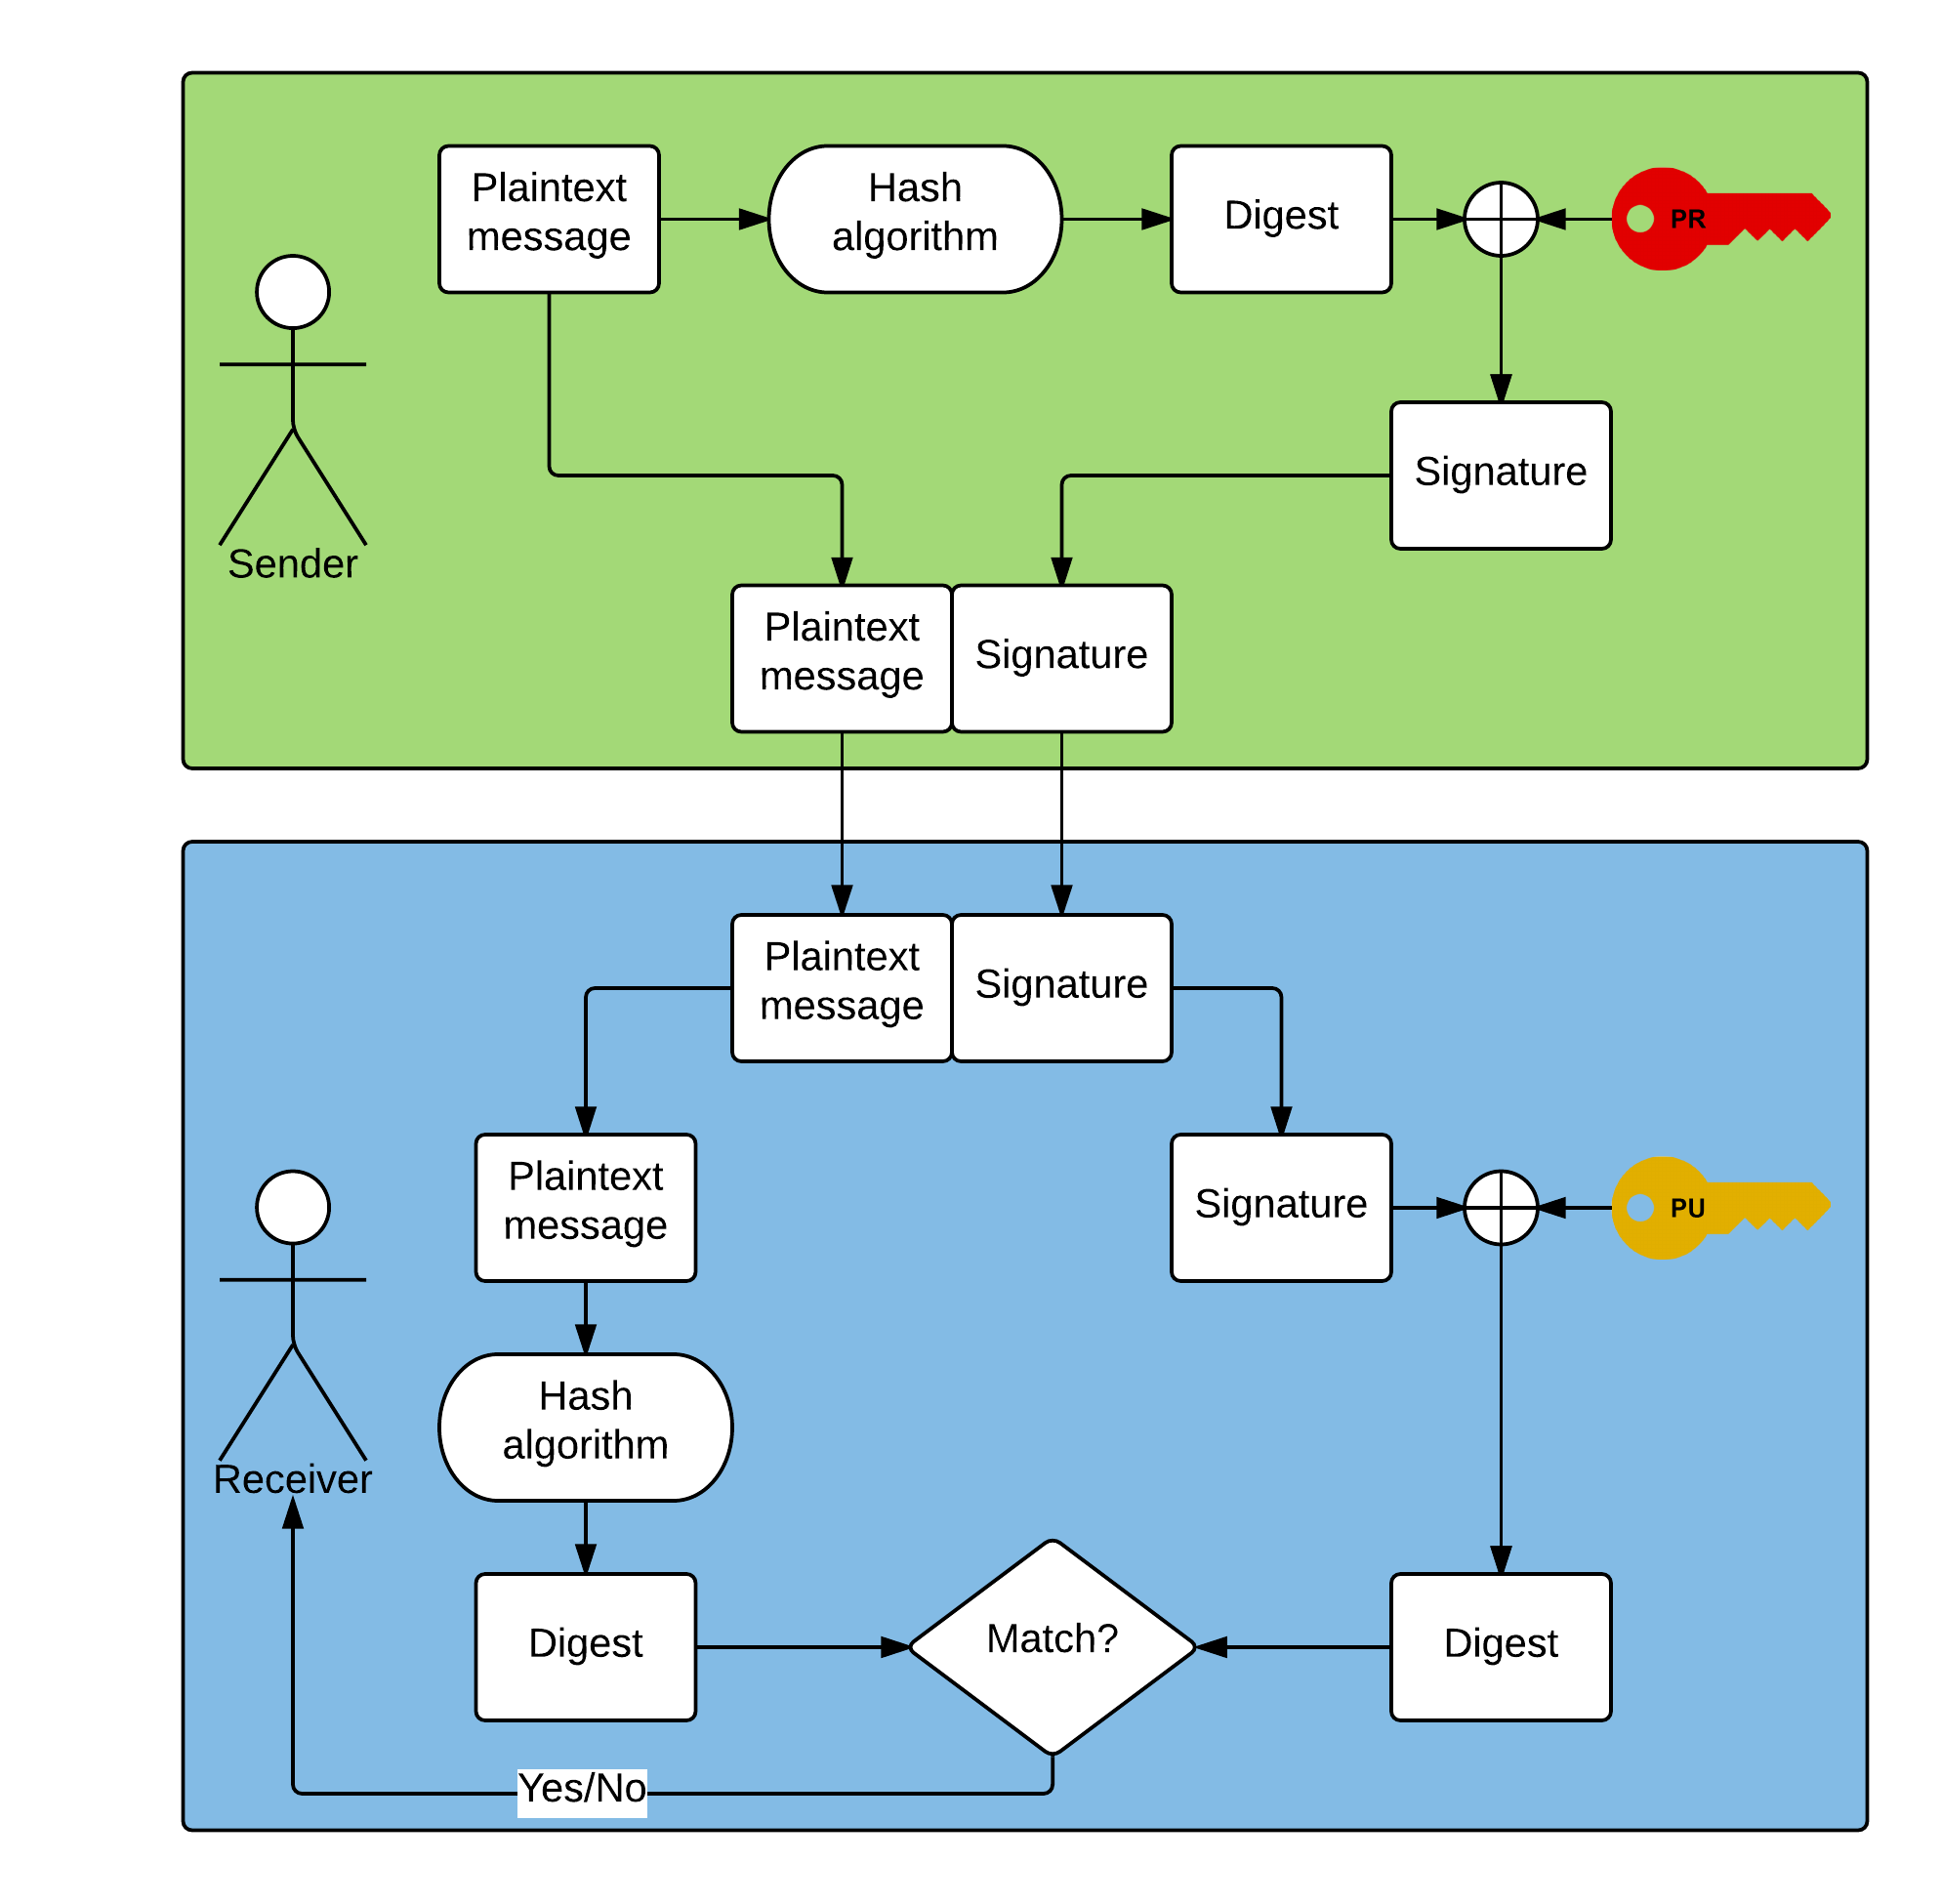
\includegraphics[width=1\textwidth]{images/signing_basic.png}
\end{figure}

\subsection{Symmetric-key cryptography}
Symmetric-key cryptography uses the same cryptographic key for both encryption and decryption. There are two main areas of application for symmetric-key cryptography; secure storage of data and secure communication. +Secure storage of data is the most straight forward of the two. An entity (user, server, etc.) generates a key, encrypts the data using the key, stores the key for future use and decrypts the data using the key whenever the entity require the data. As long as the key is stored securely and the encryption algorithm is secure the data can be stored in an unsecured environment. Secure communication using symmetric-key is very similar, but instead of the same entity decrypting the data the encrypted data is transmitted to a new entity which decrypts it using the same key. This requires the key or key generation to be a known by both parties, also known as a "shared secret". There are two methods for symmetric-key encryption/decryption. Stream ciphering takes one byte at the time and encrypts/decrypts it whereas block ciphering takes bigger chunks of data and encrypts/decrypts the data. Both methods have their own weaknesses and strenghts.

Stream ciphering is fast and relatively simplistic to implement. This along with the fact that it can encrypt byte by byte makes it very suitable for use when plaintext data comes in  unknown length and over time (streams). Areas of application includes voice chat, video feed and http communication. Disadvantages of stream ciphering is that if the algorithm is cracked then it is susceptible to insertions and modifications as well as the fact that a single plaintext symbol is represented as a single ciphertext symbol (limited alteration).

Block cipher is a more complex and requires more overhead. First of data must be divided into equal size blocks. The blocks cannot be too small as then they are prone to dictionary attacks and not too big as it will make the encryption/decryption process too resource intensive. In block cipher the block size must be fixed through the encryption process. This will often result in redundant data. For example, 200-bit plaintext with a 64-bit block size will result in three blocks of 64-bit and a fourth block with only 8 bit of "real" data and 56 bit of redundant bits. Since block ciphering uses the previous block to cipher the current block it is possible to detect tampering and faults, but this also results that data may be lost if a block becomes corrupt.


\section{Mobile threats}
Mobile threats and attack vectors are numerous and before looking into how smart cards can help mitigate an alleviate threats we will need to identify and characterize them.
\subsection{Infected device}
The most obvious threat to mobile devices is when the mobile device itself is infected with virus or malware. The type of virus or malware can vary, some are harmless and serve more as an annoyance or trying to trick the user into visiting bogus websites, but some are more malicious and will access private files and information. From a security stand-point it is a disaster if a virus or malware is able to read and modify data which is otherwise confidential.

Often the user will not know that their mobile device is infected and some viruses or malware are very hard to detect by anti-virus. The "2015 Cheetah Mobile Security Report" \cite{cheetahSec} reports that the number of viruses on Android devices exceeds over 9,5 million and that the problem is growing. Taking into concideration that the mobile device we are operating on may be infected is of the utmost importance when designing and developing applications.

\subsection{Lost or stolen device}
An attacker may gain physical access to the users mobile device through theft or simply that the user misplaced the mobile device. With physical access to the device an attacker would be able to retrive data from the device. A common defence against this is encrypting the data on the device, but this requires the keys to be stored somewhere securely. If the keys are not stored securely the result is that the data on the device will fall into the wrong hands.

\subsection{Unsecure communication channel}
\label{sec:unsecureCommunication}
Communication is a vital part of modern systems; data is sent between devices and between devices and servers. Sensitive data requires a secure communication channel which cannot be tapped into by a third party. Secure communication on public networks involves agreeing upon encryption keys which the data should be encrypted with before being sent. Encrypting the communication channel will protect against man-in-the-middle attacks, but this requires both parties to authenticate themselves as encrypting the data won't help if you are sending the data directly to the attacker. More on this in section \ref{sec:authenticationChallenges}.

\subsection{Authentication challenges}
\label{sec:authenticationChallenges}
%Are people who they say the are?
As mentioned in section \ref{sec:unsecureCommunication} a secure communication channel is useless if you are sending the data directly to the attacker. A vital part of security is being able to authenticate the parties in a transaction. If the attacker is able to impersonate another party by installing fake certificates on the mobile device or by tricking the user into communicating with the attacker the consequences can be of significance.

\subsection{Unsecure applications}
An often overlooked attack vector is badly implemented applications on the mobile device. This may include memory leaks, weak cryptography, open for code injections and plainly exposing private data to third parties. In rare cases an application with flaws may expose other applications for attacks, but there exists countermeasures to this, for instance that all applications run in their own sandbox.
